

\documentclass[12pt,twoside,a4paper]{article}

\textheight 19.7 true cm

\usepackage[dvips]{epsfig}
%\usepackage{version1}
%\usepackage{csz}
\usepackage{times}
%\usepackage{amsmath}
%\usepackage{amssymb}
\usepackage{makeidx}
\usepackage{enumerate}
%\usepackage[utf8]{inputenc}
%prova lara
%\usepackage{fancyhdr}
%\pagestylex{fancy}
%prova lara
\usepackage{multirow}
\usepackage{colortbl}
\usepackage{amsfonts}
\usepackage{amsmath}
\usepackage{tikz}
\usepackage{geometry}
\geometry{hmargin=1cm,vmargin=1cm}
\usepackage{tikz}
\def\width{15}
\def\hauteur{25}

%\usepackage{hyperref}
\usepackage[cp1250]{inputenc}
%added 2012, to make conditional checks and definition of styles
\usepackage{etoolbox}




%%%%%%%%% inputs the file that contains the definition of the commands used to create the cover file and that define if style AS2011 or AS2012 is used
%Added Lara 2012
\input{StyleAndData.tex}



%\ifthen{\value{Style}=AS2001}{\newcommand{\DocISBN}{BBB}}%{\newcommand{\DocISBN}{AAA}}
%\ifthenelse{\equal{\Style}{AS2001}}{1}{0}


%\ifdefstring{\Style}{AS2011}{\renewcommand{\DocISBN}{BBB}}{\renewcommand{\DocISBN}{AAA}} works, example for definition of styles given the value of \Stlye


%Added Lara 2009
\newcommand{\AbstractTitle}[1]{{\bf #1}\\}
\newcommand{\AbstractAuthors}[1]{{\sl #1}\\}
\newcommand{\Keyword}[1]{{\bf #1 \par \vspace{12pt}}}
%%%%%%%%%%%%%%%%%%%%%%%%%%%%%%%%%%%%%%%%%%

%%%%%%%%%%%%%%%%Added Lara 2009, from AB 2008
\newcommand{\Title}[1]{\large{\textbf{#1}}\par\vspace{12pt}}
\newcommand{\Author}[1]{
\begin{center}
\textit{#1}
\end{center}
\par}


\newcommand{\Afilliation}[1]{\small{#1}\par\vspace{2pt}}
%\newcommand{\Email}[1]{\texttt{\email{#1}}\par}
%\newcommand{\Afilliation}[1]{\small{#1}\par}
%% changed 2012, allowing two different stlyes for e-mails, each e-mail on a new line - style as2011, or all mails on the same line
\ifdefstring{\Style}{AS2011}{\newcommand{\Email}[1]{\texttt{\email{#1}}}}{\newcommand{\Email}[1]{\texttt{\email{#1}}}}
%% changed 2012, allowing two different stlyes for e-mails, each e-mail on a new line - style as2011, or all mails on the same line
%\ifdefstring{\Style}{AS2011}{\newcommand{\Email}[1]{\texttt{\email{#1}}}}{\newcommand{\Email}[1]{\texttt{\email{#1}}\par}}
%\newcommand{\AfilliationAndEmail}[1]{\begin{flushleft} #1 \end{flushleft} \par \vspace{12pt}}

%\newcommand{\AfilliationAndEmail}[1]{#1 \par \vspace{4pt}}
%\newcommand{\AfilliationAndEmail}[1]{\begin{minipage}{\linewidth} \begin{flushleft} #1  \end{minipage} \end{flushleft} \par \vspace{4pt}}

%\newcommand{\Abstract}[1]{#1 \par \vspace{36pt}}
\newcommand{\Presenting}[1]{\underline{#1}}



%2014 modifications to solve the problem related to non-left alignment of the e-mails, when they take more than one line
%as a consequence of the new command added for left alignment, the abstract text was displayed using a bigger than normal font... temporarily fixed redefining also the abstract style
\newcommand{\AfilliationAndEmail}[1]{    \begin{minipage}{\textwidth}
          \begin{flushleft}     #1   \end{flushleft}
    \end{minipage} \par \vspace{4pt}}
\newcommand{\Abstract}[1]{\vspace{8pt} \small{#1} \par \vspace{36pt}}






%modified to add topics and id,
%\newcommand{\A}[4]{
\newcommand{\A}[5]{
\begin{minipage}{\textwidth}
    \Title{#1}
    %\nopagebreak
    \Author{#2}
%\begin{minipage}{\textwidth}
%   \begin{flushleft}     \AfilliationAndEmail{#3}   \end{flushleft} \end{minipage}
%~ \vspace{4pt}
% \AfilliationAndEmail{\raggedright{#3}}

\AfilliationAndEmail{#3}

%\begin{minipage}{\linewidth}
%\begin{flushleft}
%    \AfilliationAndEmail{#3}
%\end{flushleft}
%\end{minipage}
%\par \vspace{5pt}
    %\Email{#3}
    %\Afilliation{#3}
    %\Email{#5}
    %keywords, will be removed later
    % \Keyword{#4}
    %\Abstract{#4} - put
    \Abstract{#5}
    %\pagebreak
\end{minipage}
}

\parindent 0 pt
\def\RR{\hbox{\sf I\kern-.14em\hbox{R}}}
\newcommand{\ttx}[1]{\small\sf{#1}\normalsize\rm}
\renewcommand\indexname{Index of Authors}
\makeindex

%\chead{\tiny \colorbox[rgb]{0.76,.93,1}{\hspace{2,5cm}\bf Opazovanje dejavnikov tveganja zlomov pri \v{z}enskah z
%osteoporozo v menopavzi, starih vsaj 55 let (SCOR'os)\hspace{2,5cm}}}
%\cfoot{\footnotesize \colorbox[rgb]{0.76,.93,1}{\hspace{15cm}\bf
%Applied Statistics 2008 \thepage}}


%%%% dodal Blejec %%%%%%%%%%%%%%%%%%%%%%%%%%%%%%%%%%%%%%%%%%%
\usepackage[hidelinks,
  pdfborder=0 0 0,
  pdfauthor={A. Blejec},
  pdfpagemode=UseOutline,
  pdfstartview=Fit,
  pdfpagelabels, pageanchor,
  bookmarks, bookmarksopen, bookmarksnumbered,
  citecolor= darkblue, linkcolor=blue, urlcolor=blue
]{hyperref}
\providecommand{\email}[1]{\href{mailto:#1}{\normalfont\small\texttt{#1}}}
    %%%%%%%%%%%%%%%%%%%%%%%%%%%%%%
    \oddsidemargin  0.0in
    \evensidemargin 0.0in
    \textwidth      6.0in
    \headheight     0.0in
    \topmargin      -0.75in
    \textheight=    10.0in
    %%%%%%%%%%%%%%%%%%%%%%%%%%%%%%
% ----------------------------------------------------------------
\usepackage{fancyhdr}
%% Header
\newcommand{\SetHeader}[2]{
\fancyhead{}
\fancyhead[LE,RO]{\textit{#1}}
\fancyhead[RE,LO]{ #2}
\fancyfoot{}
\fancyfoot[LE,RO]{\thepage}
\fancyfoot[RE,LO]{\small{\Footer}}
\renewcommand{\headrulewidth}{0.4pt}
\renewcommand{\footrulewidth}{0.4pt}

}

%% Session name
\newcommand{\Session}{Session name}

%% Session date
\providecommand{\Date}{Date of session}

%% Session as a section + toc
\newcommand{\Section}[1]{\clearpage \vspace{1cm}\section*{#1}
%\renewcommand{\Session}{#1}
\addcontentsline{toc}{section}{ #1}
}


%%%%%%%commands for program%%%%%%%%%%%%%%%
\newcommand{\PrSectionHeader}[4]{
\begin{tabbing}
%xxxxxxxxxxxxx\=xxxxxxxxxxxxxxxxxxxxxxxxxxxxxxxxxxxxxxxxxxxxxxxxxx\=xxxxxxxx\=xxxxxxxxxxxxx \kill
xxxxxxxxxxxxx\=xxxxxxxxxxxxxxxxxxxxxxxxxxxxxxxxxxxxx\=xxxxxxxx\=xxxxxxxxxxxxxxxxxxxxxxxxxx \kill#1  \> \bf{#2} \> #3 \> {\em #4}\\[0.1mm]
\end{tabbing}
}


%\newcommand{\PrTalk}[2]{
%\item {\bf #1}\\ \sl{#2}\\[0.1mm]
%}

%modified 2014
\newcommand{\PrTalk}[2]{
\item {\bf #1} \vspace{-15pt} \sl{#2}\\[0.1mm]
}



\raggedbottom
%% Pages as full as possible
\renewcommand{\textfraction}{0.1}
\renewcommand{\topfraction}{0.9}
\renewcommand{\floatpagefraction}{0.8}
%%
%%%% added Blejec %%%%%%%%%%%%%%%%%%%%%%%%%%%%%%%%%%%%%%%%%%%



%%% added Lara: headers also in the authors' index page - does not work!
%%%\renewcommand{\ps@plain}{\pagestyle{fancy}}




%for underscorem added by lara
%\def\us{\char`\_}
\begin{document}

%for underscore, added by Lara
%\texttt{create\us process}


%  \input{1zac.tex}

  %%%%%%%%%%%%%%%%%%%%%%%%%%%%%%% naslovnica %%%%%%%%%%%%%%%%%%%%%%%%
\thispagestyle{empty}
{\center
{\Large \bf \DocConferenceTitleA} \\[14mm]
{\LARGE \bf \DocConferenceTitleB} \\ [6mm]
{\LARGE \bf \DocYear} \\ [14mm] %[34mm]
{\large \DocTitle} \\
\begin{center} \setlength{\unitlength}{1cm}
  \includegraphics[width=130mm,angle=270, totalheight=0.55\textheight, trim=10mm 10mm 10mm 10mm,  clip]{\DocFigCover}
\end{center}
%\vfill
\DocDate \\ %[3mm]
\DocPlace \\[3mm]%[3mm]
\DocURL \\
}
\newpage

%leave an empty page so the numbering is correct also in the pdf file

\thispagestyle{empty}
%%\draft{}{}{}

%\pagestyle{myheadings}
%\markboth
%{\underline{~~~~~~~~~~~~~~~~~~~~~~~~~~~~~~~~~~~~~~~~~~~~~~~~~~~~~~~~~~~~~~~~~~~~~~~~~~~~~~~~~~~~~~~~~~~~~~~}}
%{\underline{~~~~~~~~~~~~~~~~~~~~~~~~~~~~~~~~~~~~~~~~~~~~~~~~~~~~~~~~~~~~~~~~~~~~~~~~~~~~~~~~~~~~~~~~~~~~~~~}}

~
\newpage



%%%%%%%%%%%%%%%%%%%%%%%%%%%%%%% Prva stran %%%%%%%%%%%%%%%%%%%%%%%%

\thispagestyle{empty}
\setcounter{page}{1}
{\center
{\Large \bf \DocConferenceTitleA}\\  [14mm]

{\LARGE \bf \DocConferenceTitleB} \\ [6mm]
{\LARGE \bf \DocYear} \\ [6mm]
{\Large \DocTitle}  \\ [16mm]

{\large \DocYear} \\[3mm]
{\large \DocPlace} \\[6mm]
{\large \DocURL}\\[10mm]
{\Large Organized by} \\ [3mm]
{\large \DocOrganizer} \\[10mm] %[16mm]

\vfill


%Urad vlade R Slovenije za informiranje

{\Large Supported by} \\ [3mm]
\DocSponsors }
\newpage

%%%%%%%%%%%%%%%%%%%%%%%%%%%%%%% Druga stran %%%%%%%%%%%%%%%%%%%%%%%%


\newpage
\thispagestyle{empty}

%\vspace*{11cm}
\vspace*{9cm}


\DocCenterPageTwo

\DocBottomPageTwo

\newpage


%%%%%%%%%%%%%%%%%%%%%%%%%%%%%%% Tretja stran %%%%%%%%%%%%%%%%%%%%%%%%

\thispagestyle{empty}
%\large

{\bf Scientific Program Committee}\\%[1cm]
\begin{tabbing}
%{
xxxxxxxxxxxxxxxxxxxxxxxxxxxxxxxxxxx\=xxxxxxxxxxxxxxxxxxxxxxxxxxxxxxxxxxxxxxxxxxxxxxxxxx\=xxxx \kill

\DocScientificComm
%}
\end{tabbing}

\vspace{2cm}

{\bf Organizing Committee}\\%[1cm]
\begin{tabbing}
xxxxxxxxxxxxxxxxxxxxxxxxxxxxxxxxxxx\=xxxxxxxxxxxxxxxxxxxxxxxxxxxxxxxxxxxxxxxxxxxxxxxxxx\=xxxx \kill
\DocOrganizingComm
\end{tabbing}

\noindent  \hrulefill \\

\vspace{1cm}

%\noindent  \hrulefill \\
 {
 \begin{tabbing}
 MMMMMMMMMM\=MMMMMMMMMMMMMMMMMMMMMM \kill
 {\em Published by}: \> \DocPublisher \\ %[2mm]
 {\em Edited by}: \> \DocEditors \\ %[2mm]
 {\em Printed by}: \> \DocPrinter \\
 {\em Produced using}: \> generbook R package\\
 {\em Circulation}: \> \DocCirculation \\
 \end{tabbing}
 }

\clearpage


~
\thispagestyle{empty}
\newpage


\small

%%%%%%%%restore, program overview and program
%\input{1programOverview.tex}
%\input{1program.tex}
%\input{program.tex}
%%%%%%%%restore, program overview and program

\normalsize

\newpage


\noindent\\

%%%%%%%%%%%%%%%%%% title page for the abstracts
\thispagestyle{empty}
 \begin{center}
  \Large
   \begin{flushright}
   \vspace{17cm} {\Huge \em{ \textbf{\DocTitle}}} \\ [0.5cm]
   \end{flushright}
   \normalsize
 \end{center}
%\noindent  \hrulefill \\[0.5cm]
\small
\clearpage

%%%%%%%%%%%%%%%%%%%%%%%%%%%%%%%%%%%%%%%%%
%\pagestyle{fancy}
\newpage

~



%%-------------add abstracts---------------------------

%%%%%%%%restore, program overview and program
\input{programOverview.tex}
\pagestyle{fancy}
\newpage

%\input{1program.tex}
\input{program.tex}
%%%%%%%%restore, program overview and program

\normalsize

\newpage
%\input{1prazna.tex}
%\setcounter{page}{3}

%added 2009 because of page numbering
~
\thispagestyle{empty}
%\newpage
%%%%%%%%%%%%%%%%%%%%%%%%%%

\input{abstracts.tex}

\newpage
% ------------------------------------------------- Next day -----
\renewcommand{\Date}{ }
%\addtocontents{toc}{\hfill\textbf{\Date}\\}

%% ------------------------------------------- Session start

\SetHeader{\Date}{\Session}\renewcommand{\Date}{}
\renewcommand{\Session}{}
\Section{\Session}
\SetHeader{\Date}{\Session}
%\renewcommand{\Session}{ }
%\Section{\Session}
%\SetHeader{\Date}{\Session}
%%--------------------------------------------

%\thispagestyle{empty}
%%\newpage
%%%\draft{}{}{}

%\pagestyle{myheadings}
%\markboth
%{\underline{~~~~~~~~~~~~~~~~~~~~~~~~~~~~~~~~~~~~~~~~~~~~~~~~~~~~~~~~~~~~~~~~~~~~~~~~~~~~~~~~~~~~~~~~~~~~~~~}}
%{\underline{~~~~~~~~~~~~~~~~~~~~~~~~~~~~~~~~~~~~~~~~~~~~~~~~~~~~~~~~~~~~~~~~~~~~~~~~~~~~~~~~~~~~~~~~~~~~~~~}}

~
\newpage


%added 2009 because of page numbering, cannot print index directly after the end of workshop without leaving an empty page!?!?
%\pagestyle{empty}\noindent\\  %\hrulefill \

%2014: added an empty page

%added 2009 because of page numbering, cannot print index directly after the end of workshop without leaving an empty page!?!?
\thispagestyle{empty}
%\newpage
%%\draft{}{}{}

%\pagestyle{myheadings}
%\markboth
%{\underline{~~~~~~~~~~~~~~~~~~~~~~~~~~~~~~~~~~~~~~~~~~~~~~~~~~~~~~~~~~~~~~~~~~~~~~~~~~~~~~~~~~~~~~~~~~~~~~~}}
%{\underline{~~~~~~~~~~~~~~~~~~~~~~~~~~~~~~~~~~~~~~~~~~~~~~~~~~~~~~~~~~~~~~~~~~~~~~~~~~~~~~~~~~~~~~~~~~~~~~~}}

~
\newpage




\noindent\\

%%%%%%%%%%%%%%%%%% title page for the abstracts
\thispagestyle{empty}
 \begin{center}
  \Large
   \begin{flushright}
   \vspace{17cm} {\Huge \em{ \textbf{INDEX OF AUTHORS}}} \\ [0.5cm]
   \end{flushright}
   \normalsize
 \end{center}
%\noindent  \hrulefill \\[0.5cm]
\small
%\clearpage

%%%%%%%%%%%%%%%%%%%%%%%%%%%%%%%%%%%%%%%%%
\pagestyle{empty}\noindent\\  %\hrulefill \
%\newpage
\printindex
\newpage



\pagestyle{empty}\noindent\\  %\hrulefill \

\noindent\  %\hrulefill \\
\small
%\clearpage

%% Session as a section + toc
\renewcommand{\Section}[1]{%\clearpage %\vspace{1cm}%\section*{#1}
%\renewcommand{\Session}{#1}
\addcontentsline{toc}{section}{ #1}
}



%\pagestyle{empty}\noindent\\  %\hrulefill \



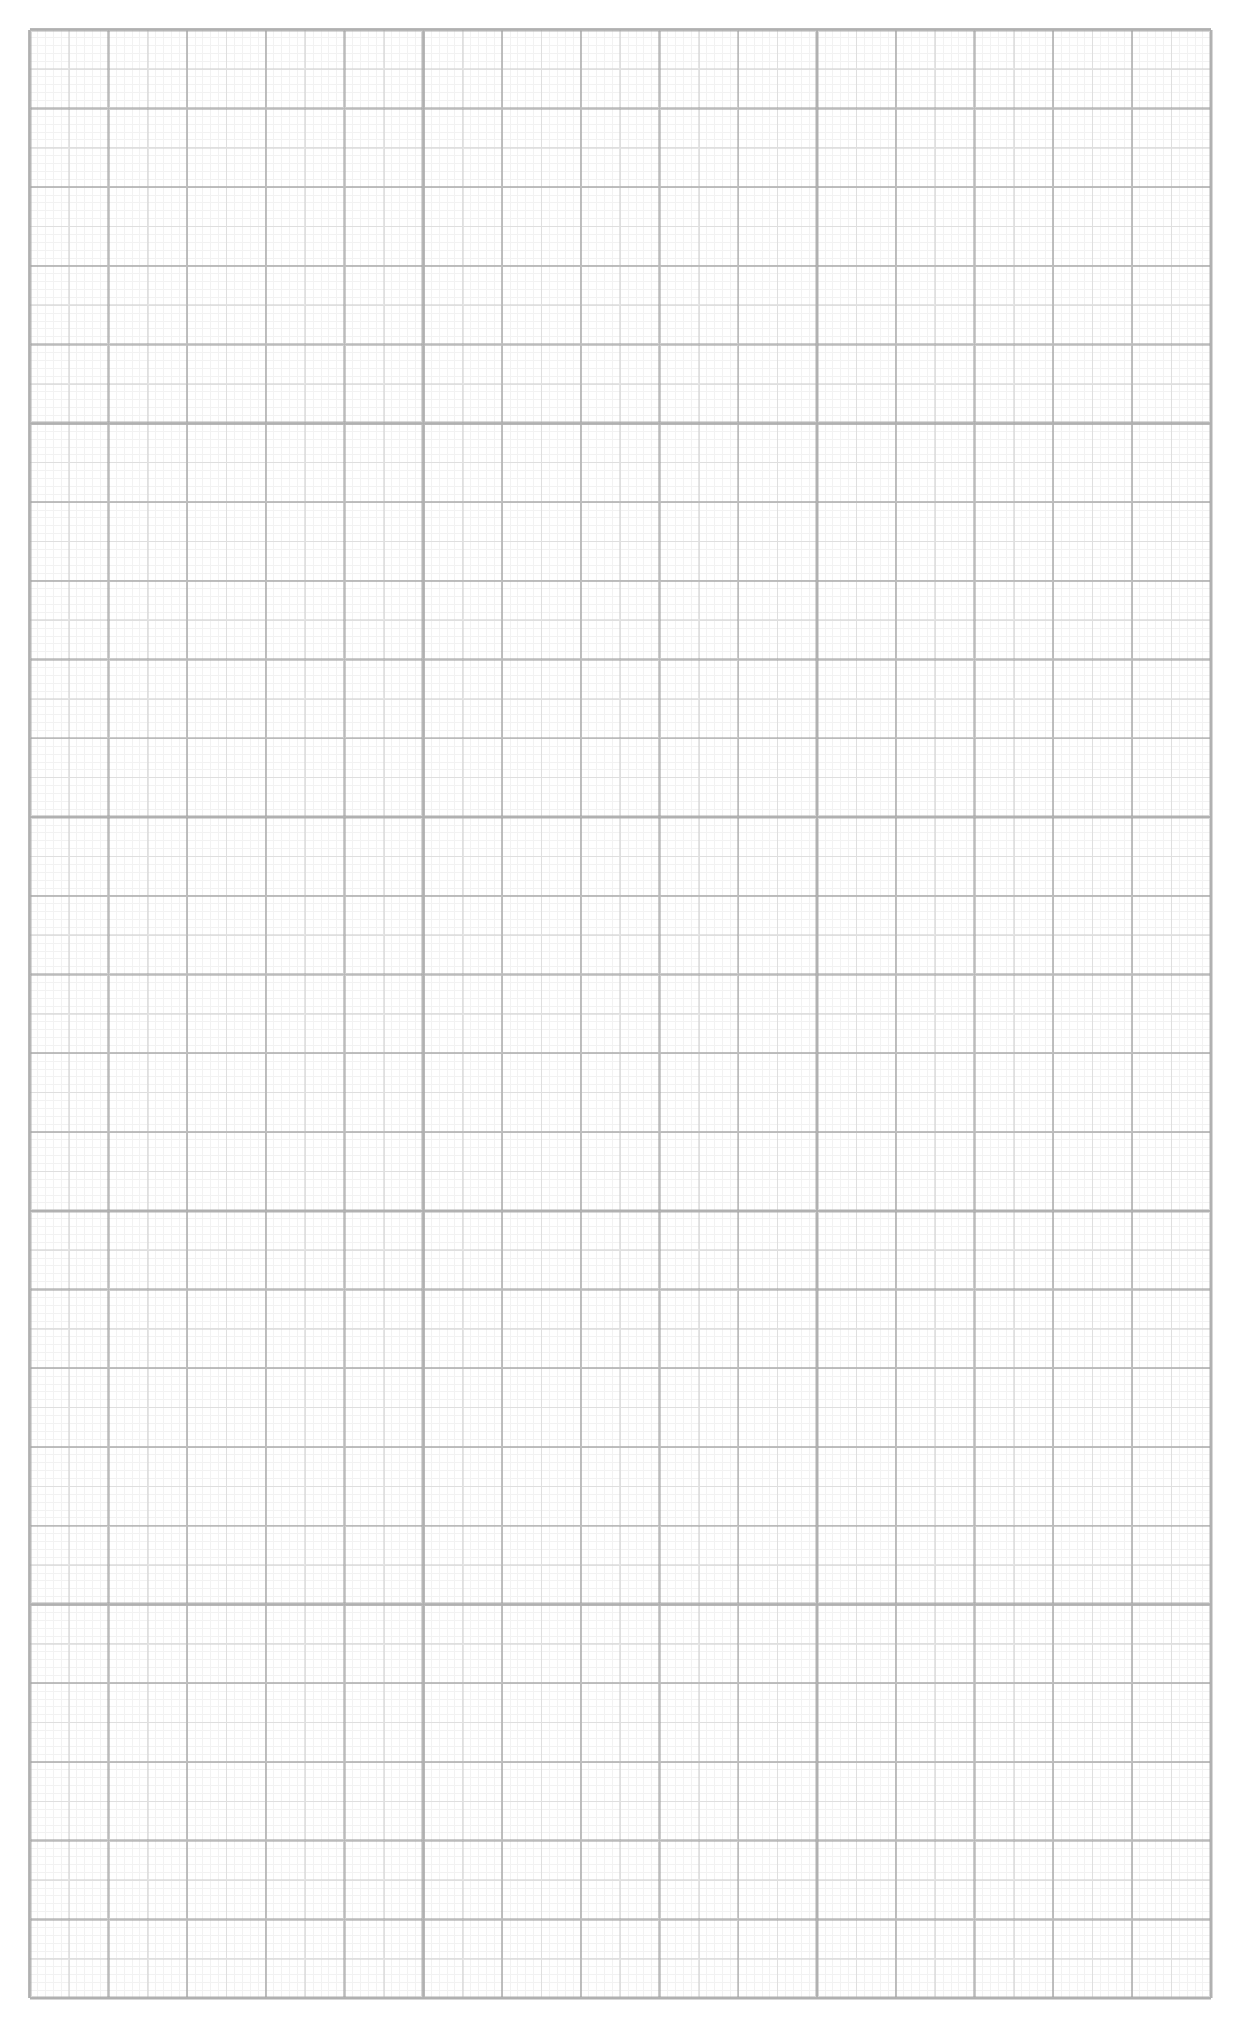
\begin{tikzpicture}[x=1cm, y=1cm, semitransparent]
\draw[step=1mm, line width=0.1mm, black!10!white] (0,0) grid (\width,\hauteur);
\draw[step=5mm, line width=0.2mm, black!20!white] (0,0) grid (\width,\hauteur);
\draw[step=5cm, line width=0.5mm, black!30!white] (0,0) grid (\width,\hauteur);
\draw[step=1cm, line width=0.3mm, black!40!white] (0,0) grid (\width,\hauteur);
\end{tikzpicture}


\pagestyle{fancy}
%\renewcommand{\Date}{}
\addtocontents{toc}{\hfill\textbf{\Date}\\}
%\renewcommand{\Session}{Notes}
\renewcommand{\Date}{Notes}
\renewcommand{\Session}{}
\Section{\Session}
\SetHeader{\Date}{\Session}



%\input{1prazna.tex}
%\input{1notes.tex}
%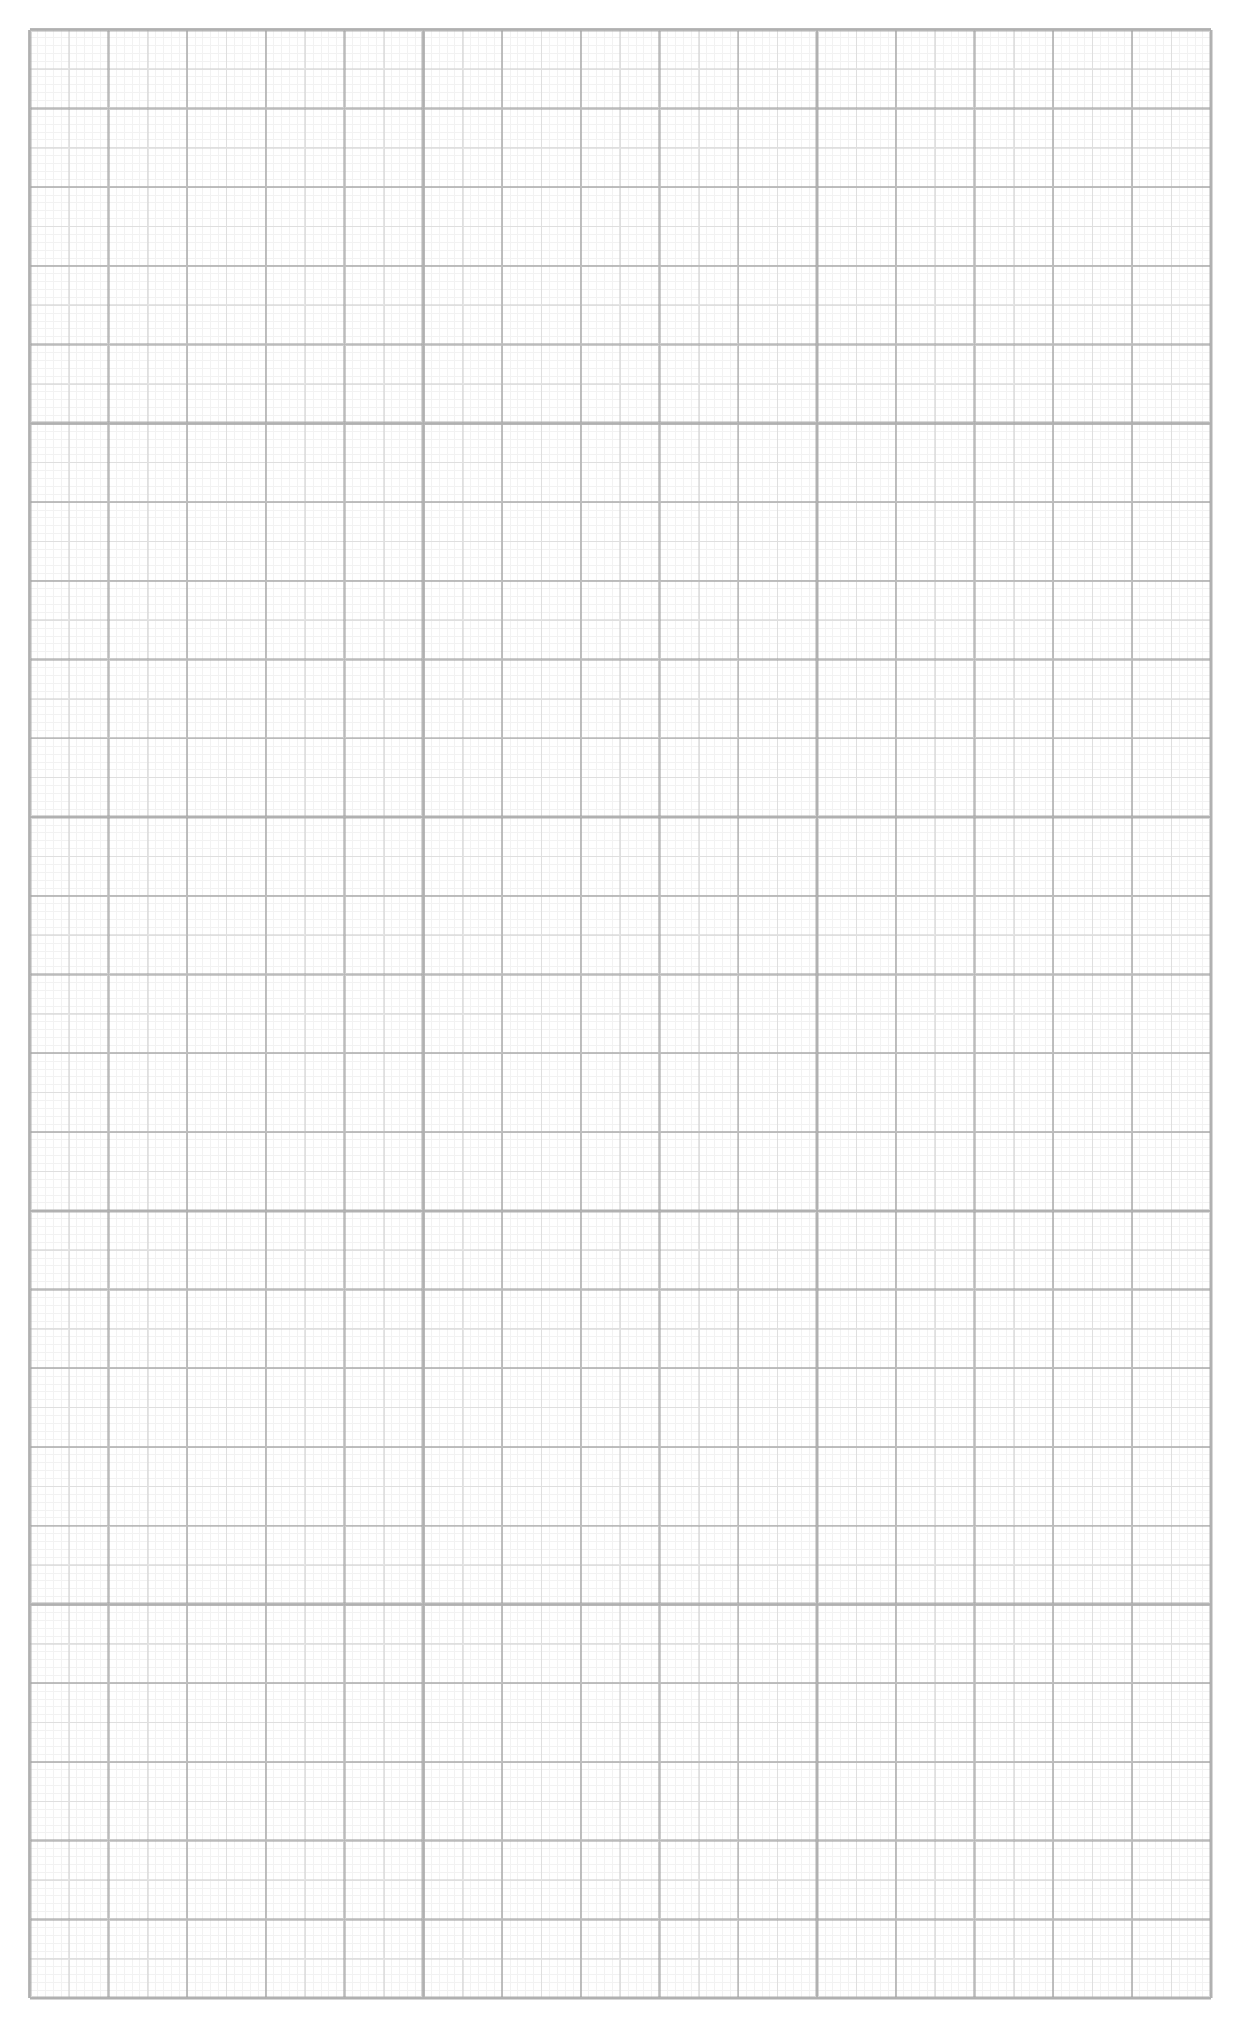
\begin{tikzpicture}[x=1cm, y=1cm, semitransparent]
\draw[step=1mm, line width=0.1mm, black!10!white] (0,0) grid (\width,\hauteur);
\draw[step=5mm, line width=0.2mm, black!20!white] (0,0) grid (\width,\hauteur);
\draw[step=5cm, line width=0.5mm, black!30!white] (0,0) grid (\width,\hauteur);
\draw[step=1cm, line width=0.3mm, black!40!white] (0,0) grid (\width,\hauteur);
\end{tikzpicture}

\clearpage
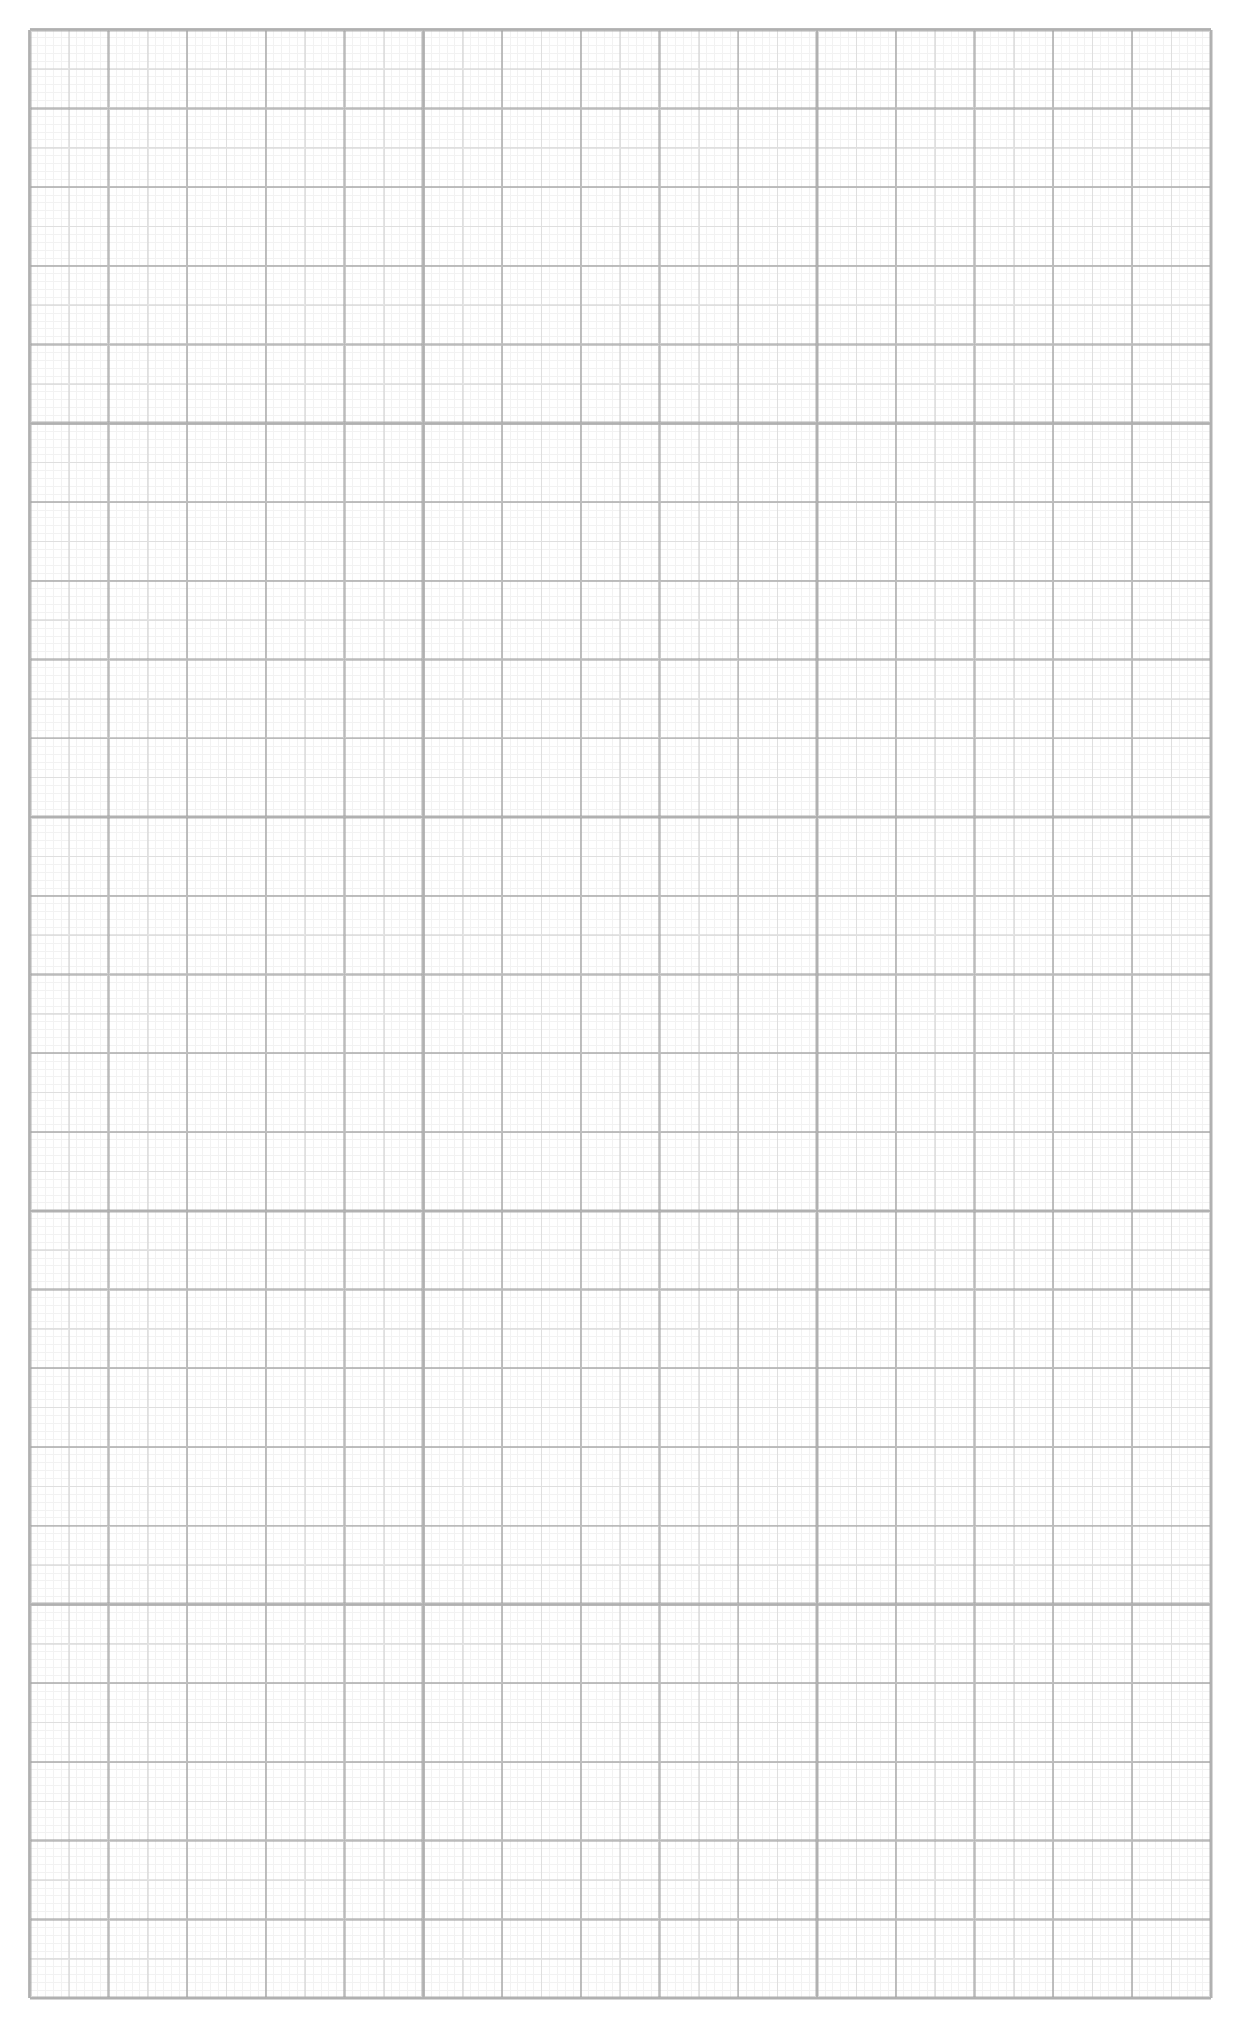
\begin{tikzpicture}[x=1cm, y=1cm, semitransparent]
\draw[step=1mm, line width=0.1mm, black!10!white] (0,0) grid (\width,\hauteur);
\draw[step=5mm, line width=0.2mm, black!20!white] (0,0) grid (\width,\hauteur);
\draw[step=5cm, line width=0.5mm, black!30!white] (0,0) grid (\width,\hauteur);
\draw[step=1cm, line width=0.3mm, black!40!white] (0,0) grid (\width,\hauteur);
\end{tikzpicture}

\clearpage
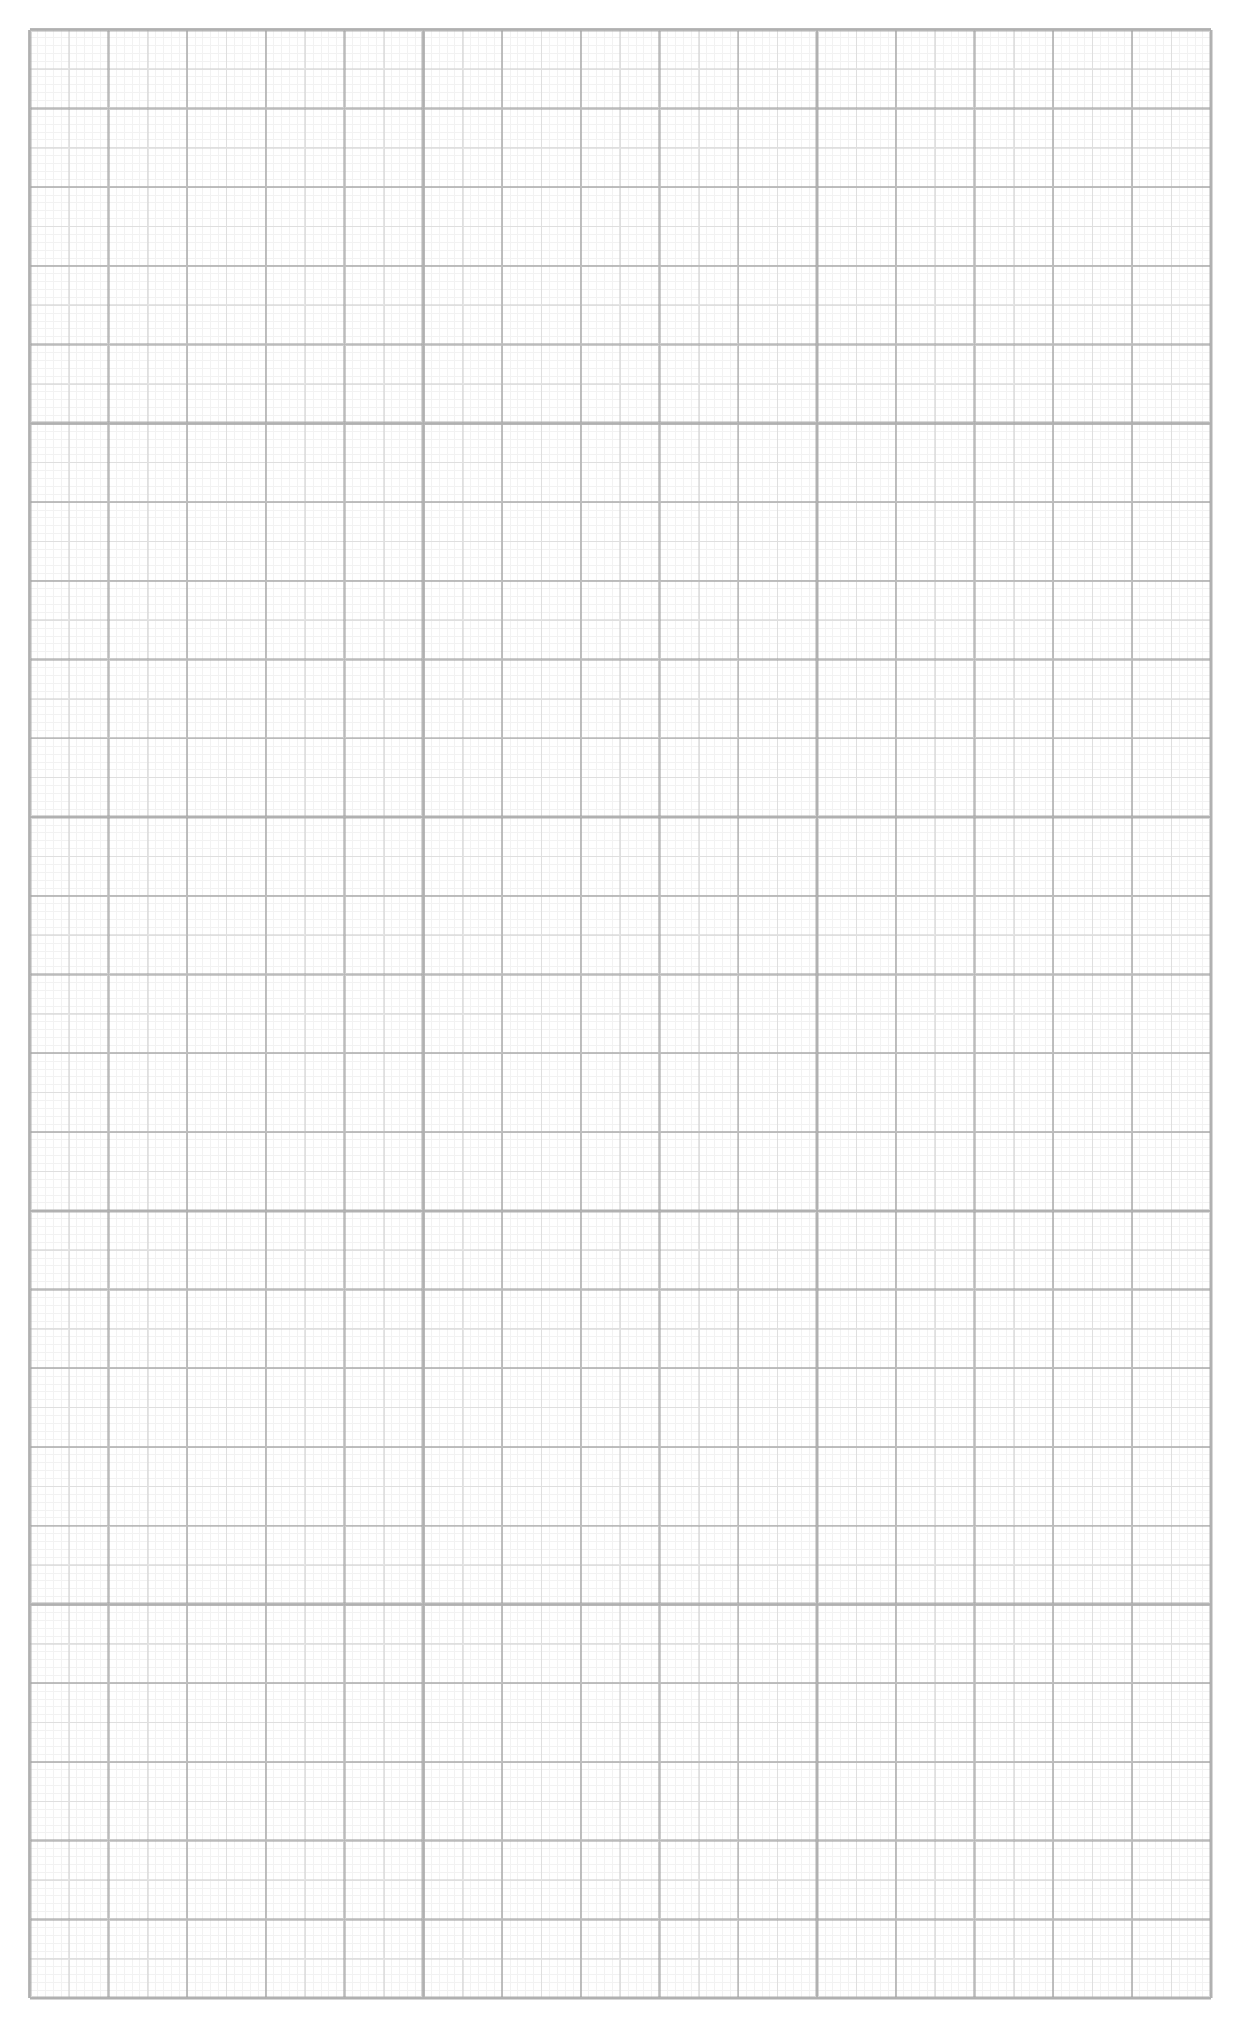
\begin{tikzpicture}[x=1cm, y=1cm, semitransparent]
\draw[step=1mm, line width=0.1mm, black!10!white] (0,0) grid (\width,\hauteur);
\draw[step=5mm, line width=0.2mm, black!20!white] (0,0) grid (\width,\hauteur);
\draw[step=5cm, line width=0.5mm, black!30!white] (0,0) grid (\width,\hauteur);
\draw[step=1cm, line width=0.3mm, black!40!white] (0,0) grid (\width,\hauteur);
\end{tikzpicture}

\clearpage
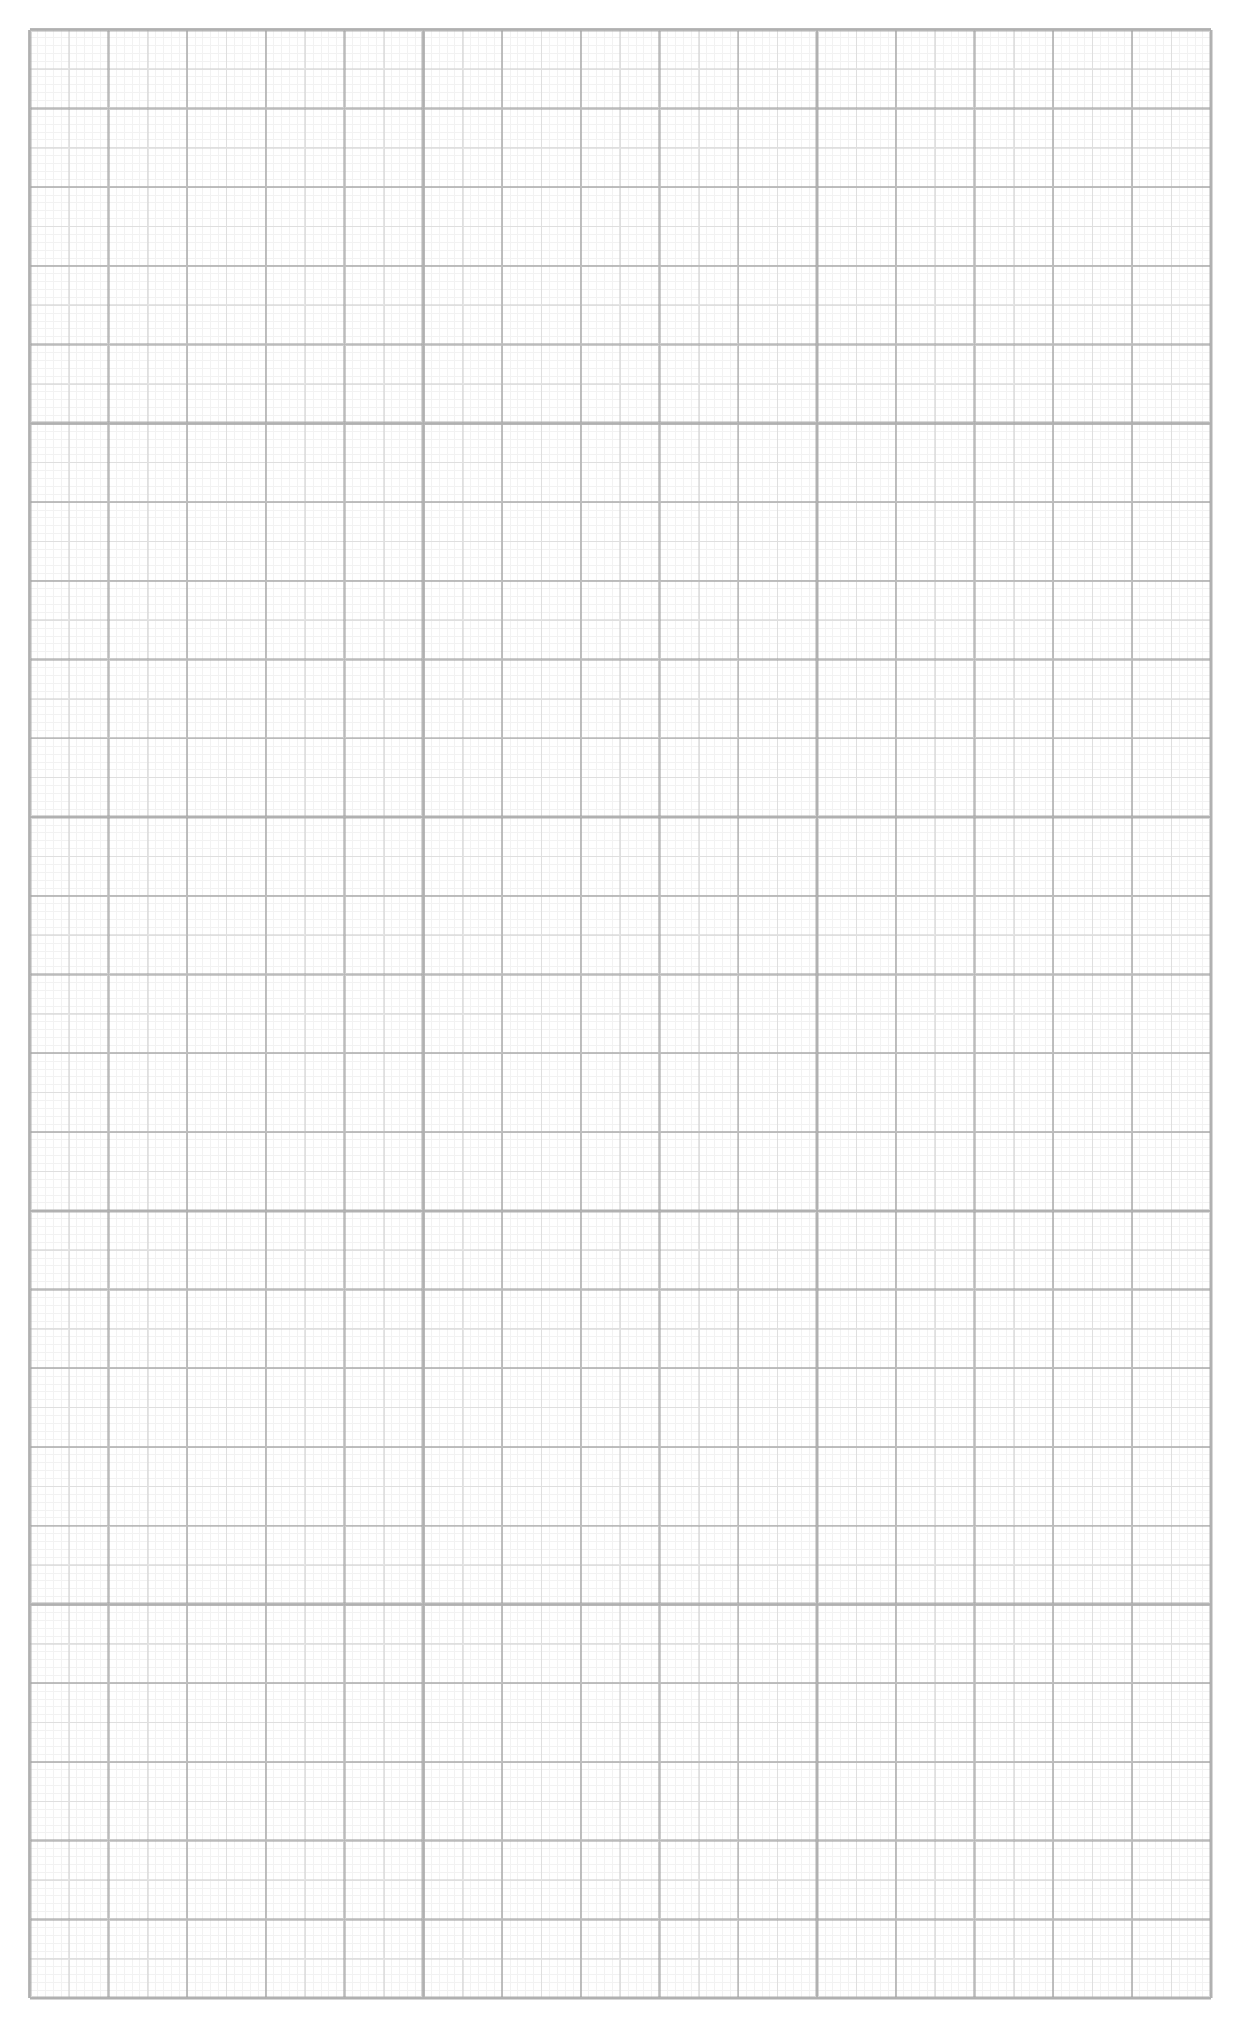
\begin{tikzpicture}[x=1cm, y=1cm, semitransparent]
\draw[step=1mm, line width=0.1mm, black!10!white] (0,0) grid (\width,\hauteur);
\draw[step=5mm, line width=0.2mm, black!20!white] (0,0) grid (\width,\hauteur);
\draw[step=5cm, line width=0.5mm, black!30!white] (0,0) grid (\width,\hauteur);
\draw[step=1cm, line width=0.3mm, black!40!white] (0,0) grid (\width,\hauteur);
\end{tikzpicture}

\clearpage
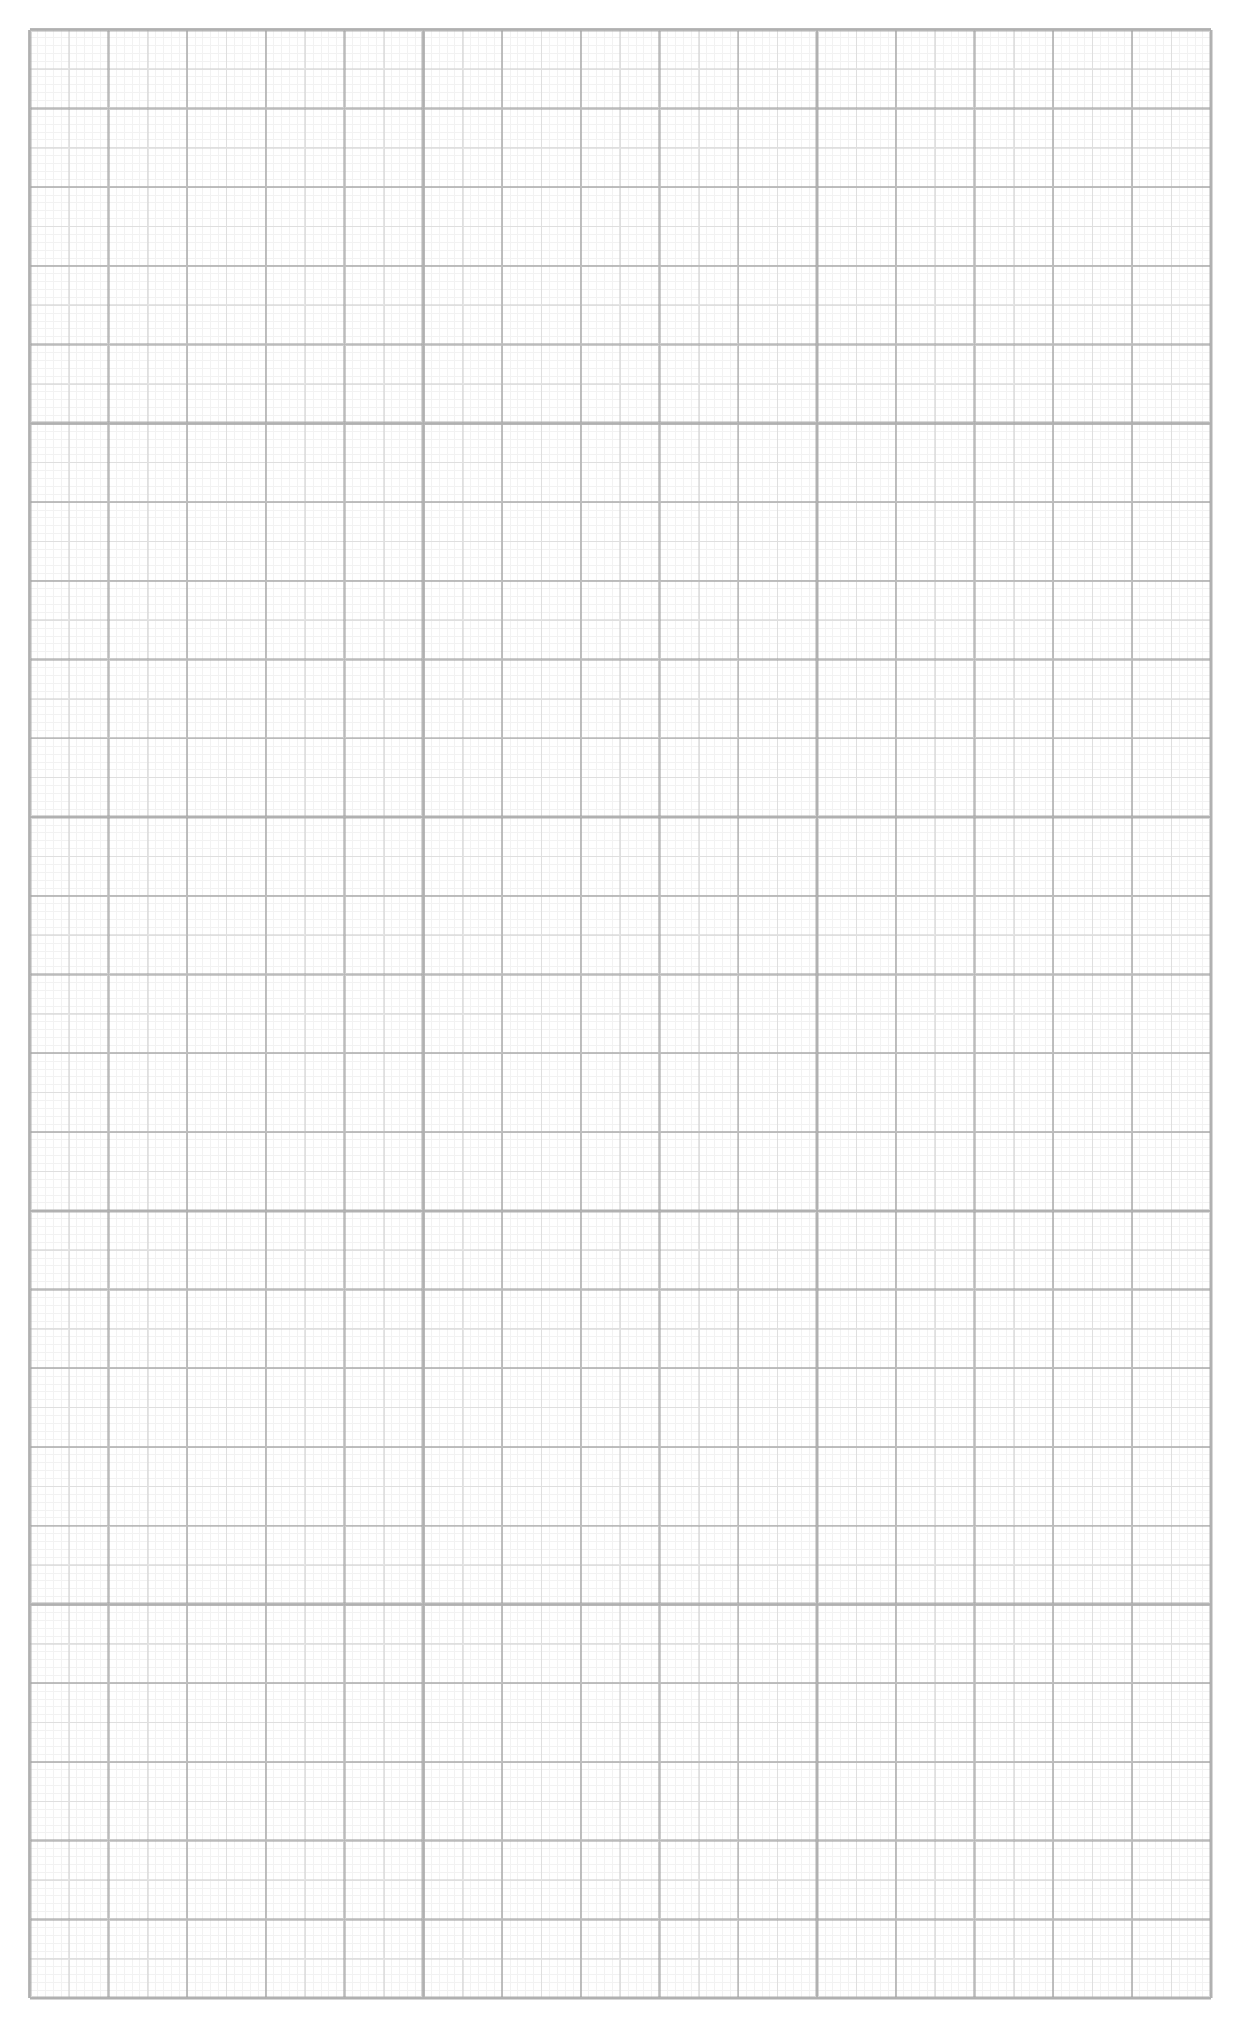
\begin{tikzpicture}[x=1cm, y=1cm, semitransparent]
\draw[step=1mm, line width=0.1mm, black!10!white] (0,0) grid (\width,\hauteur);
\draw[step=5mm, line width=0.2mm, black!20!white] (0,0) grid (\width,\hauteur);
\draw[step=5cm, line width=0.5mm, black!30!white] (0,0) grid (\width,\hauteur);
\draw[step=1cm, line width=0.3mm, black!40!white] (0,0) grid (\width,\hauteur);
\end{tikzpicture}

\clearpage
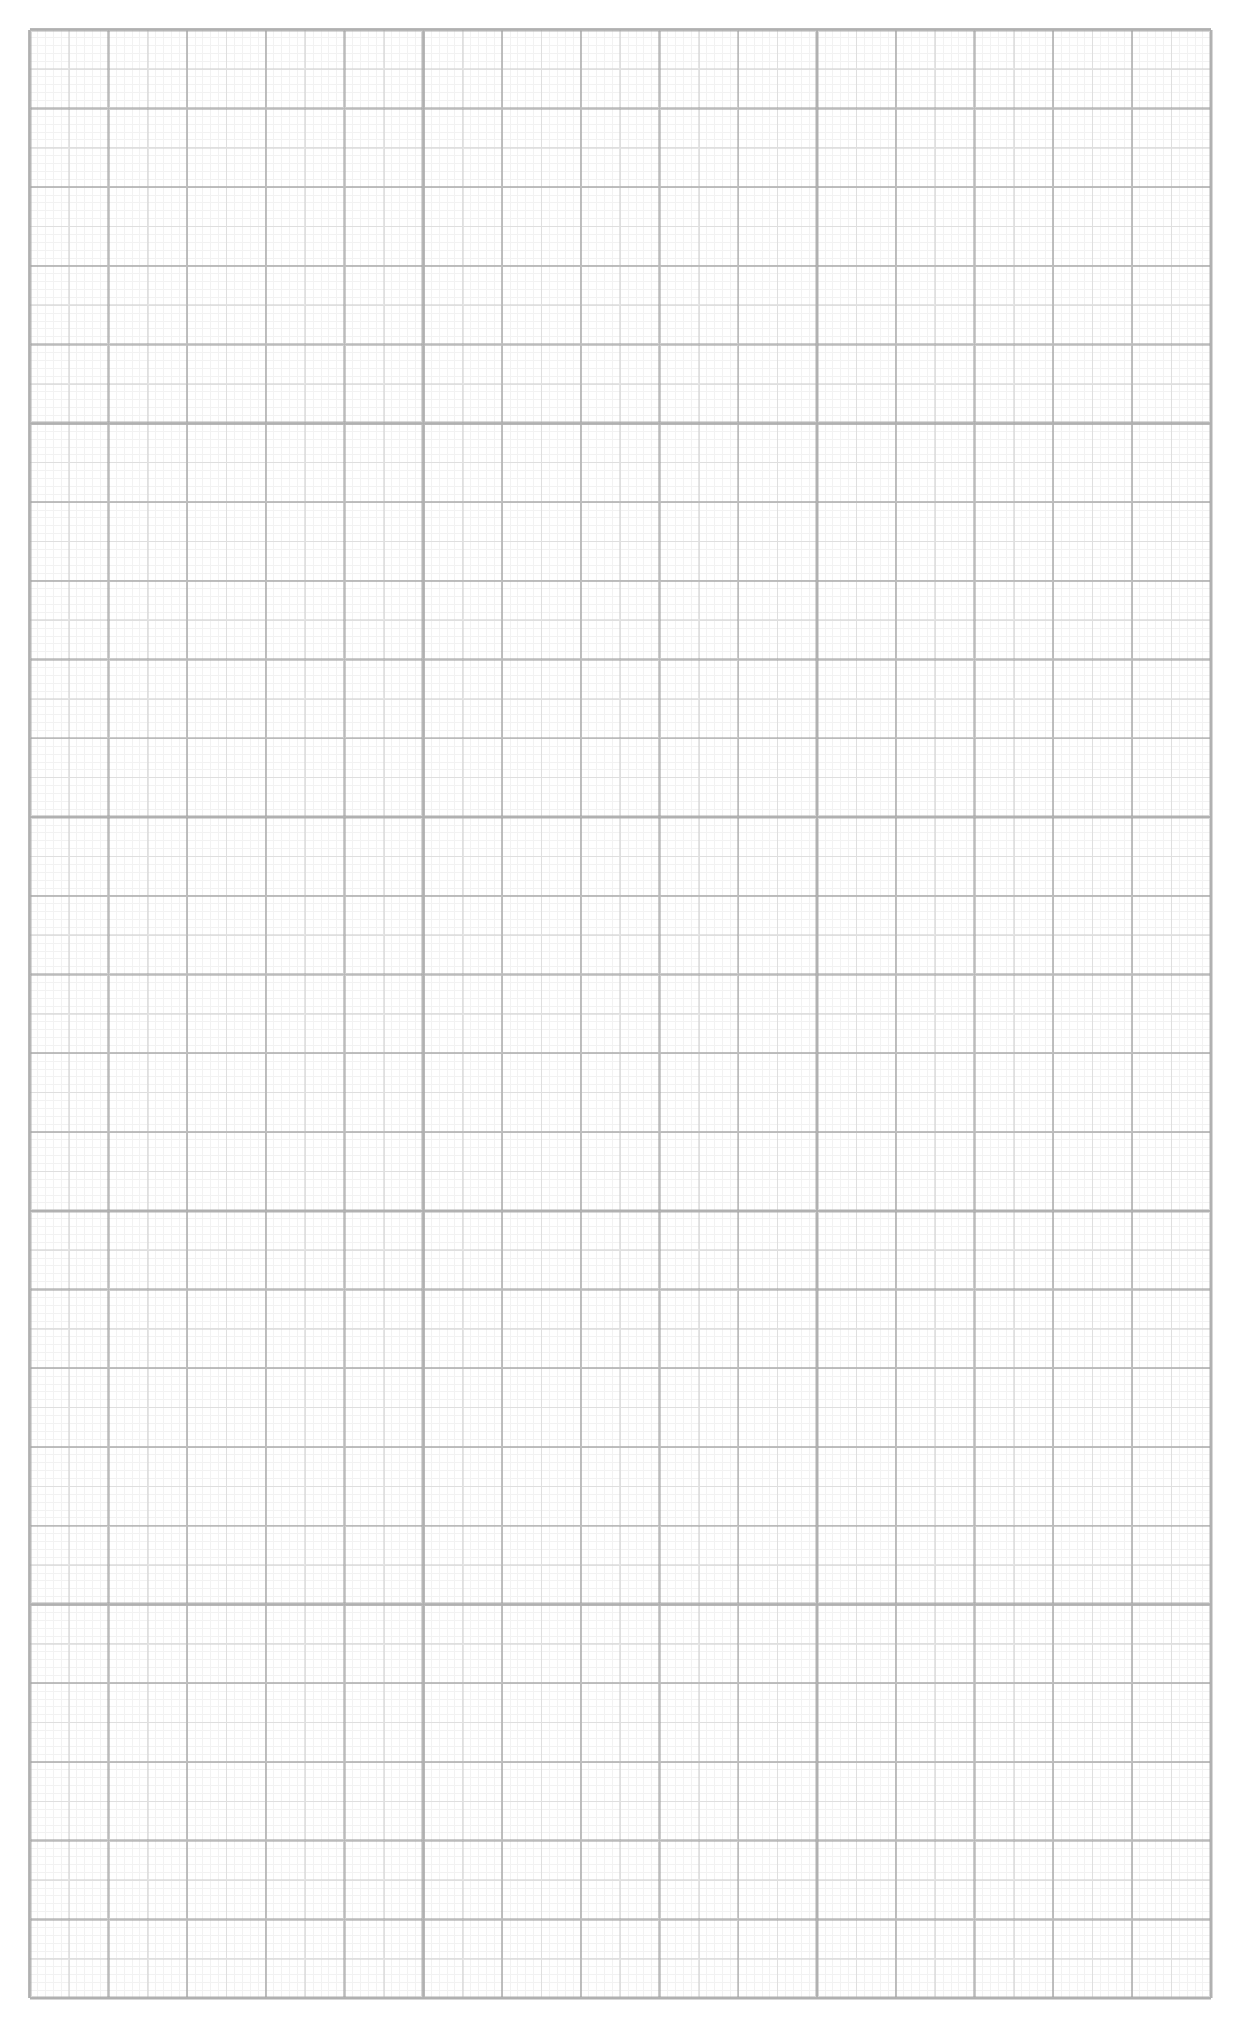
\begin{tikzpicture}[x=1cm, y=1cm, semitransparent]
\draw[step=1mm, line width=0.1mm, black!10!white] (0,0) grid (\width,\hauteur);
\draw[step=5mm, line width=0.2mm, black!20!white] (0,0) grid (\width,\hauteur);
\draw[step=5cm, line width=0.5mm, black!30!white] (0,0) grid (\width,\hauteur);
\draw[step=1cm, line width=0.3mm, black!40!white] (0,0) grid (\width,\hauteur);
\end{tikzpicture}

\clearpage
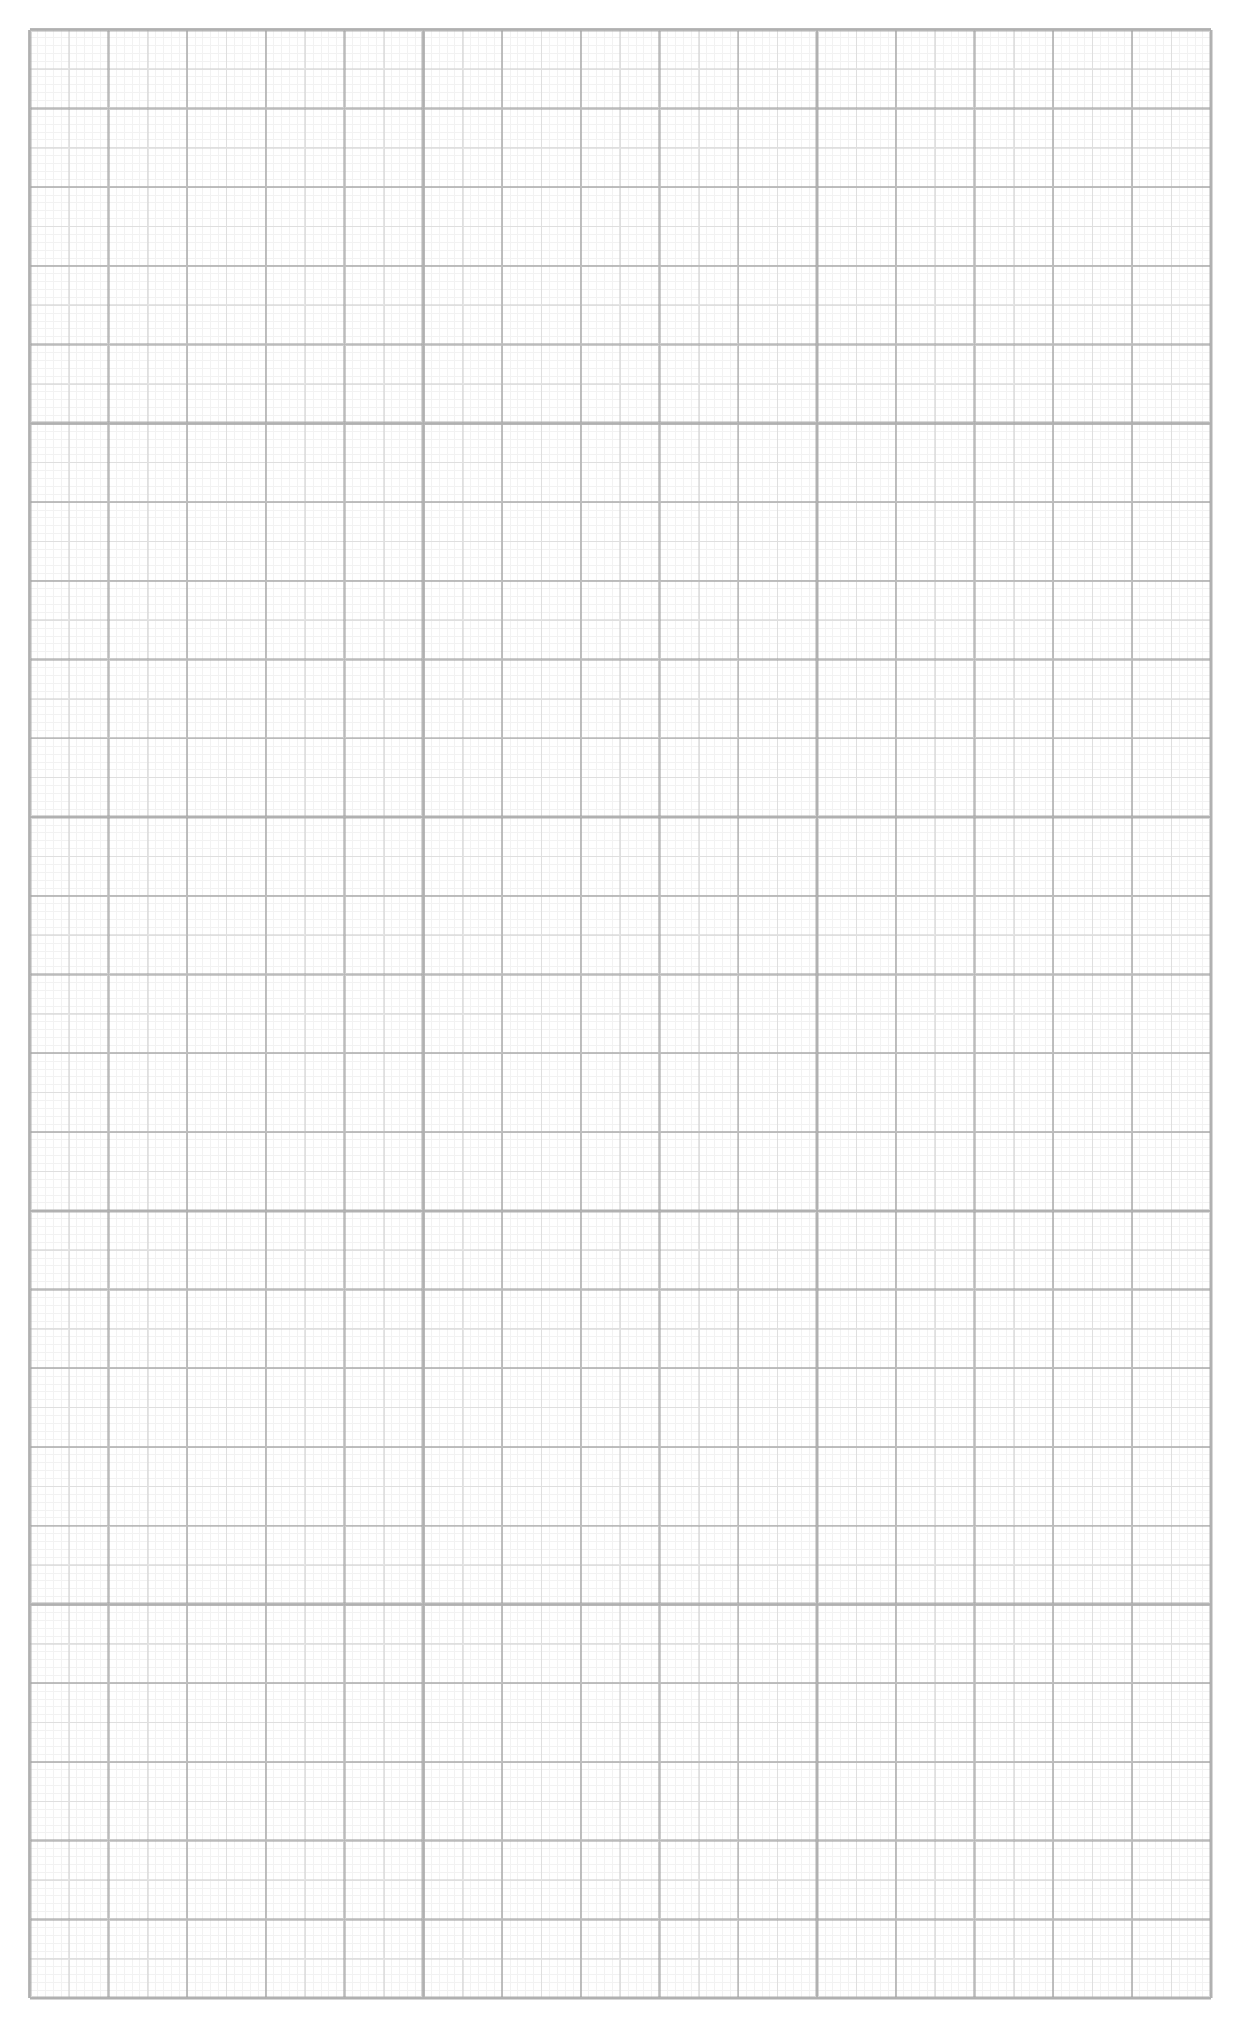
\begin{tikzpicture}[x=1cm, y=1cm, semitransparent]
\draw[step=1mm, line width=0.1mm, black!10!white] (0,0) grid (\width,\hauteur);
\draw[step=5mm, line width=0.2mm, black!20!white] (0,0) grid (\width,\hauteur);
\draw[step=5cm, line width=0.5mm, black!30!white] (0,0) grid (\width,\hauteur);
\draw[step=1cm, line width=0.3mm, black!40!white] (0,0) grid (\width,\hauteur);
\end{tikzpicture}

\clearpage



%\input{notes.tex}
%\input{notes.tex}
%\input{notes.tex}
%\input{notes.tex}

\thispagestyle{empty}
%\newpage
%%\draft{}{}{}

%\pagestyle{myheadings}
%\markboth
%{\underline{~~~~~~~~~~~~~~~~~~~~~~~~~~~~~~~~~~~~~~~~~~~~~~~~~~~~~~~~~~~~~~~~~~~~~~~~~~~~~~~~~~~~~~~~~~~~~~~}}
%{\underline{~~~~~~~~~~~~~~~~~~~~~~~~~~~~~~~~~~~~~~~~~~~~~~~~~~~~~~~~~~~~~~~~~~~~~~~~~~~~~~~~~~~~~~~~~~~~~~~}}

~
\newpage



\pagestyle{fancy}
\renewcommand{\Date}{}
\addtocontents{toc}{\hfill\textbf{\Date}\\}
\renewcommand{\Session}{}
\Section{\Session}
\SetHeader{\Date}{\Session}


\begin{center}
\Huge {\em SUPPORTED BY}\\
%\bigskip
%\begin{figure}[!h]
 %\setlength{\unitlength}{1cm}
  %\begin{picture}(10,20)(0,0)
  %  \put(0,0){
\includegraphics[width=100mm]{sponsors}}
  %\end{picture}
%\end{figure}
%\noindent  \hrulefill \\
\vspace{3cm}
\hspace{1.5cm} \includegraphics{sponsors2014}
%%%\newline
%\noindent  \hrulefill \\
\small
\end{center}







\end{document}
